\begin{enumerate}[label=\arabic*.,ref=\theenumi]
%
\item A counter is constructed with three $D$ flip-flops. The input-output pairs are named $\brak{D_0, Q_0}$, $\brak{D_1, Q_1}$, and $\brak{D_2, Q_2}$, where the subscript $0$ denotes the least significant bit. The output sequence is desired to be the Gray-code sequence $000, 001, 011, 010, 110, 111, 101$, and $100$, repeating periodically. Note that the bits are listed in the $Q_2$  $Q_1$  $Q_0$ format. The combinational logic expression for $D_1$ is
%
	\begin{multicols}{2}
\begin{enumerate}
    \item $Q_2 Q_1 Q_0$
    \item $Q_2 Q_0 + Q_1 \Bar{Q_0}$
    \item $\Bar{Q_2} Q_0 + Q_1 \Bar{Q_0}$
    \item $Q_2 Q_1 + \Bar{Q_2} \Bar{Q_1}$
\end{enumerate}
	\end{multicols}
\hfill(GATE EE 2021)
%
\item Implement a 4-stage ripple counter utilizing flip-flops.
\label{gate-ee-2022-29}
\hfill (GATE EE 2022)
%
\iffalse
\item 
 The Clock (clk) frequency provided to the circuit 
in	\figref{fig:PropagationDelay}
is $500$ MHz.
%
	\begin{figure}[H]
    \centering
    \resizebox{0.75\columnwidth}{!}{%
    \input{figs/figggss.tex}
		}
    \caption{Propagation Delay}
	\label{fig:PropagationDelay}
\end{figure}
Starting from the initial value of the flip-flop outputs $Q2Q1Q0 =1 1 1$ with $D2=1$, find the time after which $Q2Q1Q0=1 0 0$. 
\hfill(GATE EC 2021)
\fi
%
\item In the circuit in 
	\figref{fig:GATE EC 2021},
\label{prob:gate-ec-46.2021}
the clock (Clk) frequency provided to the circuit is 500MHz.
Starting from the initial value of the flip-flop outputs $Q2Q1Q0 =111$ with $D2=1$, fine the time after which $Q2Q1Q0 = 1 0 0$. 
\hfill (GATE EC 2021)
%
	\begin{figure}[H]
    \centering
    \resizebox{0.75\columnwidth}{!}{%
\begin{tikzpicture}
\ctikzset{                                   
logic ports=ieee,                   
logic ports/scale=0.5               
}                                    
\draw(-1.3,-0.56)node[xor port,anchor=out](x) {};  
%Drawing flip-flops
\draw (-1.3,-1.3) rectangle (0,0);
\draw(-1,-0.6) node{$D2$};
\draw(0.7,-1.3) rectangle (2,0);
\draw(1,-0.6) node{$D1$};
\draw(2.7,-1.3) rectangle (4,0);
\draw(3,-0.6) node{$D0$};
%connecting them
\draw(0,-0.6) -- (0.7,-0.6);
\draw(2,-0.6) -- (2.7,-0.6);
\draw(4,-0.6) -- (4.35,-0.6);
%drawing clk
\draw(-1.5,-2) node[above]{$clk$} -- (3.35,-2);
%connecting clk 
\draw(-0.65,-2) -- (-0.65,-1.3);
\draw(1.35,-2) -- (1.35,-1.3);
\draw(3.35,-2) -- (3.35,-1.3);
%drawing clk edges
\draw(-0.5,-1.3) -- (-0.65,-1.1) -- (-0.8,-1.3);
\draw(1.2,-1.3) -- (1.35,-1.1) -- (1.5,-1.3);
\draw(3.2,-1.3) -- (3.35,-1.1) -- (3.5,-1.3);
%drawing Q2,Q1,Q0
\draw(0.35,-0.6) --(0.35,0.3);
\draw(2.35,-0.6) --(2.35,0.35);
\draw(4.35,-0.6) --(4.35,0.9);
\draw(4.35,0.9) -- (-3,0.9);
\draw(0.35,0.3) -- (-2.5,0.3);
\draw(x.in 2) -|(-3,-0.7)to[short](-3,0.9);
\draw(x.in 1) -|(-2.5,-0.3)to[short](-2.5,0.3);
\draw(0.35,0.5)node{$Q2$};
\draw(2.35,0.45)node{$Q1$};
\draw(4.35,1)node{$Q0$};
\end{tikzpicture}
	}
    \caption{}
	\label{fig:GATE EC 2021}
\end{figure}


\item  
\label{prob:gate IN 17}
For the $3$-bit binary counter shown in 
\figref{fig:lcd}, the output increments at every positive 
transition in the clock (CLK). Assume ideal diodes and the starting state of the counter as 
$000$. If output high is $1 V$ and output low is $0 V$, find the current $I$ (in mA) flowing through the 
$50 \Omega$ resistor during the $5$th clock cycle (up to one decimal place).

\hfill(GATE IN 2018)
\begin{figure}[H]
\centering
\includegraphics[width=0.75\columnwidth]{ide/7474/figs/pic.png}
\caption{}
\label{fig:lcd}
\end{figure}
\item
\label{prob:gate CS 22}
Consider the sequential circuit shown in \figref{fig:wert}, where both flip-flops used are positive
    edge-triggered D flip-flops.
The number of states in the state transition diagram of this circuit that have a transition back to the same state on some value of ``in" is \rule{1cm}{0.1pt}.
   \hfill(GATE IN 2018)
\begin{figure}[H]
        \centering      
        \includegraphics[width=0.75\columnwidth]{ide/7474/figs/wert.jpg}
        \caption{}    
        \label{fig:wert}
    \end{figure}
%
   \item Implement the synchronous sequential circuit shown below 
in \figref{fig:gate EC 2023}
	   with a clock frequency of $500 Hz$. 
\hfill(GATE EC 2023)
\label{prob:GATE EC 2023}
	\begin{figure}[H]
    \centering
    \resizebox{0.75\columnwidth}{!}{%
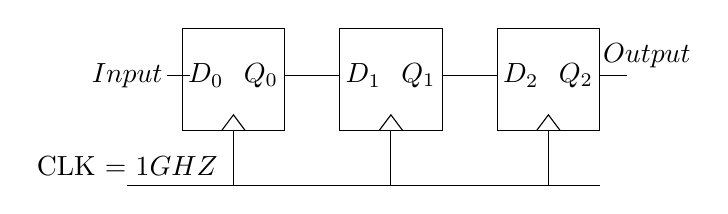
\begin{tikzpicture}
\ctikzset{                                  
    logic ports=ieee,                   
    logic ports/scale=0.5               
}                                    
%
% Drawing flip-flops
\draw (-1.3,-1.3) rectangle (0,0);
\draw(-1,-0.6) node{$D_0$};
\draw(-0.3,-0.6) node{$Q_0$};
\draw(0.7,-1.3) rectangle (2,0);
\draw(1,-0.6) node{$D_1$};
\draw(1.7,-0.6) node{$Q_1$};
\draw(2.7,-1.3) rectangle (4,0);
\draw(3,-0.6) node{$D_2$};
\draw(3.7,-0.6) node{$Q_2$};

% Connecting them
\draw(0,-0.6) -- (0.7,-0.6);
\draw(2,-0.6) -- (2.7,-0.6);
\draw(4,-0.6) -- (4.35,-0.6);
\draw(-1.2,-0.6) -- (-1.5,-0.6);

% Drawing clk
\draw(-2,-2) node[above]{CLK = $1GHZ$ } -- (3.35,-2);

% Connecting clk
\draw(-0.65,-2) -- (-0.65,-1.3);
\draw(1.35,-2) -- (1.35,-1.3);
\draw(3.35,-2) -- (3.35,-1.3);
\draw(3.35,-2) -- (4,-2);

% Drawing clk edges
\draw(-0.5,-1.3) -- (-0.65,-1.1) -- (-0.8,-1.3);
\draw(1.2,-1.3) -- (1.35,-1.1) -- (1.5,-1.3);
\draw(3.2,-1.3) -- (3.35,-1.1) -- (3.5,-1.3);

% Drawing Q2, Q1, Q0
\draw(0.35,-0.3)node{};
\draw(2.35,-0.35)node{};
\draw(4.6,-0.35)node{$ Output $};
\draw(-2,-0.6)node{$ Input $};
\end{tikzpicture}
	}
		\caption{}
\label{fig:gate EC 2023}
\end{figure}
\item In a given sequential circuit
	in \figref{fig:GATE EC 2023},
	 initial states are $Q1 = 1$ and $Q2 = 0$. For a clock frequency of $1 MHz$, find the frequency of signal $Q2$ in kHz (rounded off to the nearest integer).
\hfill(GATE EC 2023)
   % 
	\begin{figure}[H]
    \centering
    \resizebox{0.5\columnwidth}{!}{%
\begin{tikzpicture}              

%Drawing flip-flops
\draw (1.6,1.9) node {D Flip Flop};
\draw (0,0)--(3,0)--(3,4)--(0,4)--(0,0);
\draw(0.5,3.5) node{$D_1$};
\draw(2.5,3.5) node{$Q_1$};
\draw(2.5,0.5) node{$\bar{Q_1}$};
\draw(3.1,0.5) node{$\circ$};

\draw (8.6,1.9) node {D Flip Flop};
\draw(7,0)--(7,4)--(10,4)--(10,0)--(7,0);
\draw(7.5,3.5) node{$D_2$};
\draw(9.5,3.5) node{$Q_2$};
\draw(9.5,0.5) node{$\bar{Q_2}$};
\draw(10.1,0.5) node{$\circ$};

%connecting them
\draw(3.2,0.5)--(4.0,0.5);
\draw(10.2,0.5)--(10.9,0.5);
\draw(7.0,3.5)--(6.0,3.5);
\draw(4.0,0.5) -- (6.0,3.5);
\draw(10.0,3.5) -- (10.9,3.5);
\draw(4.0,3.5) --(3.0,3.5);

\draw(-1.1,-1.2)-- (8.5,-1.2);

%drawing clk
\draw (-1.0,-1.7)node{CLK =1Mhz};


%connecting clk 
\draw(1.5,-1.2) -- (1.5,0.0);
\draw(8.5,-1.2) -- (8.5,0.0);

%drawing clk edges
\draw(1.1,0.0) -- (1.48,0.4) -- (1.9,0.0);
\draw(8.1,0.0) -- (8.48,0.4) -- (8.9,0.0);

% Drawing Q2, D1,
\draw(10.9,3.5)--(10.9,5.4);
\draw(10.9,5.4)--(-1.0,5.4);
\draw(-1.0,5.4)--(-1.0,3.5);
\draw(0,3.5)--(-1.0,3.5);
\end{tikzpicture}
	}
    \caption{}
	\label{fig:GATE EC 2023}
\end{figure}
%
\item Find the decimal equivalent of $ABCD$
	in
\figref{fig:Gate_question.png}.
\hfill{(EE GATE 2023)}
%
\begin{figure}[H]
 \centering
\includegraphics[width=0.5\columnwidth]{ide/7474/figs/Gate_question.png}
\caption{}
\label{fig:Gate_question.png}
\end{figure}
%
\item 
Consider a sequential digital circuit consisting of T flip-flops and D flip-flops as shown in 
\figref{fig:Flip-Flop}.
 CLKIN is is the clock input to the circuit. At the beginning,Q1,Q2 and Q3 have values 0,1 and 1, respectively.
Which of the given values of \((Q_1, Q_2, Q_3)\) can NEVER be obtained with this digital circuit?
\hfill(GATE CS 2023)
	\begin{multicols}{4}
\begin{enumerate}
    \item ${(0,0,1)}$
    \item ${(1,0,0)}$
    \item ${(1,0,1)}$
    \item ${(1,1,1)}$
\end{enumerate}
	\end{multicols}
%
	\begin{figure}[H]
    \centering
    \resizebox{0.75\columnwidth}{!}{%
\input{ide/7474/figs/fig.tex}
		}
\caption{}
\label{fig:Flip-Flop}
\end{figure}
\item In the circuit shifter in 
\figref{fig:cricuit Digram},
the initial binary content of the shift register $A$ is $1101$ and that of shift register $B$ is $1010$ The shift registers are positive edge triggered, and the gates have no delay.
when the shift control is high, which of the following are legitimate combinations of binary content of the shift registers $A$ and $B$ in any clock pulse?
\hfill{(GATE IN 2023)}
%
\begin{multicols}{2}
\begin{enumerate}
\item $A= 1101,B=1101$
\item $A=1110,B=1001$
\item $A=0101,B=1101$
\item $A=1010,B=1111$
\end {enumerate}
\end{multicols}
\begin{figure}[H]
\centering
\includegraphics[width=0.75\columnwidth]{ide/7474/figs/Gate.png}
\caption{}
\label{fig:cricuit Digram}
\end{figure}
%
\item For the circuit shown
in
			\figref{fig:new_gate},
	 the clock frequency is $f_0$ and the duty cycle is $25\%$. For the signal at the Q output of the Flip-Flop,\hfill(GATE EC 2022)
			\begin{multicols}{2}
			\begin{enumerate}
			\item frequency is $\frac{{f_0}}{4}$ and duty cycle is $50\%$
			\item frequency is $\frac{{f_0}}{4}$ and duty cycle is $25\%$
			\item frequency is $\frac{{f_0}}{2}$ and duty cycle is $50\%$
			\item frequency is ${f_0}$ and duty cycle is $25\%$
		\end{enumerate}
			\end{multicols}
		\begin{figure}[H]
			\centering
			\includegraphics[width=0.75\columnwidth]{ide/7474/figs/gate_image_new.jpg}
			\caption{Circuit}
			\label{fig:new_gate}
		\end{figure}
\item The digital circuit shown in \figref{fig:GATEIN202236.png}
\hfill(GATE IN 2022)
\begin{figure}[H]
  \centering
  \includegraphics[width=0.75\columnwidth]{ide/7474/figs/GATEIN202236.png}
  \caption{}
  \label{fig:GATEIN202236.png}
\end{figure}
			\begin{multicols}{2}
 \begin{enumerate}
 \item is a divide-by-$5$ counter
 \item is a divide-by-$7$ counter
 \item is a divide-by-$8$ counter
 \item does not function as a counter due to disjoint cycles of states 
\end{enumerate}
			\end{multicols}
%
 \item Given below 
in
		      \figref{fig:GATE-IN2021}
	 is the diagram of a synchronous sequential circuit with one $J-K$ flip-flop and one $T$ flip-flop with their outputs denoted as $A$ and $B$ respectively, with $J_{A}=\brak{A^{\prime}+B^{\prime}}$, $K_{A}=(A+B)$ and $T_{B}=A$. Starting from the initial state $\brak{AB=00}$, the sequence of states $\brak{AB}$ visited by the circuit is
\hfill(GATE IN 2021)
			\begin{multicols}{2}
		  \begin{enumerate}
          \item $00 \rightarrow 01 \rightarrow 10 \rightarrow 11 \rightarrow 00 
          \dots $
          \item $00 \rightarrow 10 \rightarrow 01 \rightarrow 11 \rightarrow 00 
          \dots $
          \item $00 \rightarrow 10 \rightarrow 11 \rightarrow 01 \rightarrow 00 \dots $
          \item $00 \rightarrow 01 \rightarrow 11 \rightarrow 00 \dots $
      \end{enumerate}
			\end{multicols}
	\begin{figure}[H]
    \centering
    \resizebox{0.75\columnwidth}{!}{%
		      \input{figs/jkff.tex}
		      }
		      \caption{}
		      \label{fig:GATE-IN2021}
	      \end{figure}
  \item Consider the $D$-Latch shown in 
	\figref{fig:GATE-EC2017},
		which is transparent when its clock input $CK$ is high and has zero propagation delay. In the figure, the clock signal $CLK1$ has $50\%$ duty cycle and $CLK2$ is a one fifth period delayed version of $CLK1$. The duty cycle at the output of the latch in percentage is \rule{1cm}{1pt}.
  \hfill(GATE-EC2017)
	\begin{figure}[H]
    \centering
    \resizebox{0.75\columnwidth}{!}{%
			      \input{ide/7474/figs/fig22245.tex}
	}
    \caption{}
	\label{fig:GATE-EC2017}
\end{figure}
\item A $4$-bit shift register circuit configured for right-shift operation, i.e.\\ $D_{in} \rightarrow A, A \rightarrow B, B \rightarrow C, C \rightarrow D$, is shown
	in \figref{fig:GATE-EC-2017}.
 If the present state of the shift register is $ABCD = 1101$, the number of clock cycles required to reach the state $ABCD = 1111$ is
\rule{1cm}{0.1pt}.
\hfill (GATE EC 2017)
	\begin{figure}[H]
    \centering
    \resizebox{0.4\columnwidth}{!}{%
	\input{ide/7474/figs/fig22246.tex}
		}
 	\caption{}
	\label{fig:GATE-EC-2017}
\end{figure}
%
\item In the circuit shown
	in \figref{fig:GATE-EC2019,25},
the clock frequency is 12 KHz. The frequency of the signal at $Q2$ is  \rule{1cm}{0.1pt} KHz.

		\hfill(GATE EC 2019)
%%\end{enumerate}
	\begin{figure}[H]
    \centering
    \resizebox{0.75\columnwidth}{!}{%
			\input{ide/7474/figs/fig1.tex}
			}
    \caption{}
	\label{fig:GATE-EC2019,25}
\end{figure}
%
 \item The circuit shown in 
	\figref{fig:GATE-IN2019,12}
below uses ideal positive edge-triggered synchronous $J-K$ flip flops with outputs $X$ and $Y$. If the initial state of the output is $X=0$ and $Y=0$ just before the arrival of the first clock pulse, the state of the output just before the arrival of the second clock pulse is
              \hfill(GATE IN 2019)
			\begin{multicols}{2}
\begin{enumerate}
    \item $X=0$, $Y=0$
    \item $X=0$, $Y=1$
    \item $X=1$, $Y=0$
    \item$X=1$, $Y=1$
\end{enumerate}
			\end{multicols}
	\begin{figure}[H]
    \centering
    \resizebox{0.75\columnwidth}{!}{%
    \input{ide/7474/figs/fig7.tex}
	}
    \caption{}
	\label{fig:GATE-IN2019,12}
\end{figure}
%
	\item The digital circuit shown in Fig. \ref{fig:2004-gate-ee-68} generates a modified clockpulse at the output. Sketch the output waveform.
\label{prob:2004-gate-ee-68}
\hfill (GATE EE 2004)
%
\begin{figure}[H]
	\centering
	\includegraphics[width=0.75\columnwidth]{figs/2004-gate-ee-68.jpg}
	\caption{}
\label{fig:2004-gate-ee-68}
\end{figure}
%
\item Consider a $4$-bit counter constructed out of four flip-flops. It is formed by connecting the J and K inputs to logic high and feeding the Q output to the clock input of the flip-flop in 
	\figref{fig:GATE-PH2020,30}.
 The input signal to the counter is a series of square pulses and the change of state is triggered by the falling edge. At time $t=t_0$ the outputs are in logic low state (Q0 = Q1 = Q2 = Q3 = 0). Then at $t=t_1$, the logic state of the outputs is 
		               \hfill(GATE PH 2020)
			\begin{multicols}{2}
\begin{enumerate}
\item  Q0 = 1, Q1 = 0, Q2 = 0 and Q3 = 0 
\item  Q0 = 0, Q1 = 0, Q2 = 0 and Q3 = 1
\item  Q0 = 1, Q1 = 0, Q2 = 1 and Q3 = 0
\item  Q0 = 0, Q1 = 1, Q2 = 1 and Q3 = 1
\end{enumerate}
			\end{multicols}
\begin{figure}[H]
    \centering
    \resizebox{0.75\columnwidth}{!}{%
\input{ide/7474/figs/fig10.tex}
	}
    \caption{}
	\label{fig:GATE-PH2020,30}
\end{figure}
%
\iffalse
\item Two T-flip flops are interconnected as shown in 
	\figref{fig:GATEIN2020-40}.
 The present state of the flip flops are: A = 1, B = 1. The input x is given as $1, 0, 1$ in the next three clock cycles. The decimal equivalent of $\brak{ABy}_{2}$ with A being the MSB and y being the LSB, after the $3_{rd}$ clock cycle is $\underline{\hspace{2cm}}$.
\hfill (GATE IN 2020)
	\begin{figure}[H]
    \centering
    \resizebox{0.5\columnwidth}{!}{%
\input{ide/7474/figs/fig15.tex}
	}
    \caption{}
	\label{fig:GATEIN2020-40}
\end{figure}
%
\fi
\item A 2-bit synchronous counter using two J-K flip flops is shown
in \figref{fig:gate_in_2018_44}.
 The expression for the inputs to the J-K flip flops are also shown in the figure. The output sequence of the counter starting from $Q_{1}Q_{2} = 00$ is
\hfill (GATE IN 2018)
			\begin{multicols}{2}
\begin{enumerate}
\item $00 \rightarrow 11 \rightarrow 10 \rightarrow 01 \rightarrow 00 \hdots $
\item $00 \rightarrow 01 \rightarrow 10 \rightarrow 11 \rightarrow 00 \hdots $
\item $00 \rightarrow 01 \rightarrow 11 \rightarrow 10 \rightarrow 00 \hdots $
\item $00 \rightarrow 10 \rightarrow 11 \rightarrow 01 \rightarrow 00 \hdots $
\end{enumerate}
			\end{multicols}
%
\begin{figure}[H]
\centering
    %\resizebox{0.75\columnwidth}{!}{%
    \resizebox{\columnwidth}{!}{%
\input{ide/7474/figs/gate_in_2018_44.tex}
	}
	\caption{}
\label{fig:gate_in_2018_44}
\end{figure}
%
 \item Which of the following statements is true about digital circuit shown in 
	\figref{fig:GATE-EE-2018,36}?
 \hfill (GATE EE 2018)
%
	\begin{figure}[H]
    \centering
    \resizebox{0.75\columnwidth}{!}{%
\begin{circuitikz}
\draw (0,0)node[left]{$f_{in}$} to[short,*-] (8,0);
\draw (0.5,0) to (0.5,1);
\draw (0.5,1) to (1,1);
\draw (1,0.65) to (1,3);
\draw (1,3) to (3,3);
\draw (3,3) to (3,0.65);
\draw (3,0.65) to (1,0.65);
\draw (1,2.65) node[right]{D}to (0.5,2.65);
\draw (0.5,2.65) to (0.5, 5);
\draw (0.5,5) to (4,5);
\draw (3,2.65) node[left]{Q}to (5,2.625) node[right]{D};
\draw (5,0.65) to (5,3);
\draw (5,3) to (7,3);
\draw (7,3) to(7,0.65);
\draw (5,0.65) to (7,0.65);
\draw (4,0) to (4,1);
\draw (4,1) to (5,1);
\draw (7,2.65) node[left]{Q} to (9,2.65) node[right]{D};
\draw (9,0.65) to (9,3);
\draw (9,3) to (11,3);
\draw (11,3) to (11,0.65);
\draw (11,0.65) to (9,0.65);
\draw (8,0) to (8,1);
\draw (8,1) to (9,1);
\draw (11,2.65) node [left]{Q} to [short,-*](12,2.65) node[right]{$f_{out}$};
\draw (8,2.65) to (8,4.5);
\draw (8,4.5) to (6.25,4.5);
\draw (11.5,2.65) to (11.5,5.5);
\draw (11.5,5.5) to (6.25,5.5);
\draw (1,1.25) to (1.25,1);
\draw (1.25,1) node[right]{C} to (1,0.75);
\draw (5,1.25) to (5.25,1);
\draw (5.25,1) node[right]{C} to (5,0.75);
\draw (9,1.25) to (9.25,1);
\draw (9.25,1) node[right]{C} to (9,0.75);
% nand
\draw (4,5) node[rotate=180,nand port,scale=1.77](nand){};
\end{circuitikz}
	}
    \caption{}
	\label{fig:GATE-EE-2018,36}
\end{figure}
%
\begin{enumerate}
\item It can be used  for dividing the input frequency by $3$.
\item  It can be used  for dividing the input frequency by $5$.
\item  It can be used  for dividing the input frequency by $7$.
\item  It cannot be reliably used as frequency divider due to 
 disjoint internal cycles.
 \end{enumerate}
%
 \item In the circuit shown below, a positive edge-triggered $D$ Flip-Flop is used for sampling input data $D_{in}$ using clock $CK$. The $XOR$ gate outputs $3.3$ volts for logic HIGH and $0$ volts for logic LOW levels. The data bit and clock periods are equal and the value of $\triangle T/ T_{CK} = 0.15$, where the parameters $\triangle T$ and $T_{CK}$ are shown in 
	\figref{fig:GATE EC 2018,46}.
 Assume that the Flip-Flop and the $XOR$ gate are ideal.
 If the probability of input data bit ($D_{in}$) transition in each clock period is $0.3$, the average
    value (in volts, accurate to two decimal places) of the voltage at node $X$, is \rule{1cm}{0.1pt}.
%
\hfill (GATE EC 2018)
	\begin{figure}[H]
    \centering
    \resizebox{0.75\columnwidth}{!}{%
			\input{ide/7474/figs/ckt.tex}
	}
    \caption{}
	\label{fig:GATE EC 2018,46}
\end{figure}
   % 
 \item Assume that all the digital gates in the circuit shown in 
	\figref{fig:GATE EC 2016}
are ideal,the resistor $R$=$10k\Omega $ and the supply voltages is $5V$. The $D$ flip-flops $D_1,D_2,D_3,D_4$ and $D_5$ are intialized with logic values $0,1,0,1,$ and $0,$ respectively. The clock has a $30\%$ duty cycle.
The average power dissipated in the resistor $R$ is \rule{1cm}{0.1pt}.
\hfill{(GATE EC 2016)}
% 
	\begin{figure}[H]
    \centering
    \resizebox{0.75\columnwidth}{!}{%
    \begin{circuitikz}[scale=0.8]

      \tikzset{flipflop AB/.style={flipflop,
    flipflop def={t1=D,t6=Q,td={\texttt{CLK}}},
 }}
     \draw(0,0) node[flipflop AB](D1){D1} ;
     \draw(3,0) node[flipflop AB](D2){D2};
     \draw(6,0) node[flipflop AB](D3){D3};
     \draw(9,0) node[flipflop AB](D4){D4};
     \draw(12,0) node[flipflop AB](D5){D5};
     \draw (D1.pin 6) --  (D2.pin 1);
     \draw (D2.pin 6) --  (D3.pin 1);
     \draw (D3.pin 6) --  (D4.pin 1);
     \draw (D4.pin 6) --  (D5.pin 1);
     \draw (15.2,5) node[or port] (or) {};
     \draw (or.in 1) node[left]{};
     \draw (or.in 2) node[left]{};
     \draw (or.out) node[right]{};
     \draw (D5.pin 6) -- (or.in 2);
     \draw (-3,1.05) -- (D1.pin 1);
     \draw (-3,1.05) -- (-3,-3);
     \draw (-3,-3) --   (13.45,-3);
     \draw (13.4,-3) -- (D5.pin 6);
     \draw (7.3,5.3) -- (or.in 1);
     \draw (7.3,1.05) -- (7.3,5.25);
     \draw (0,-2) -- (0,-1.5);
     \draw (0,-2) -- (3,-2);
     \draw (3,-2) -- (6,-2);
     \draw (6,-2) -- (9,-2);
     \draw (9,-2) -- (12,-2);
     \draw (15.4,5) to[R, l=$10\, \text{k}\Omega$] (15.4,0);
     \draw (15.38,0) node[ground]{};
     \draw (-1,-2) node[left](q){$Clock$};
     \draw (q) -- (0,-2);
\end{circuitikz}
	}
    \caption{}
	\label{fig:GATE EC 2016}
\end{figure}
\iffalse
\item The circuit shown in 
\figref{fig:2019-gate-in-12}
below uses ideal positive edge-triggered synchronous J-K flip flops with outputs X and Y. If the initial state of the output is X=0 and Y=0, just before the arrival of the first clock pulse, the state of the output just before the arrival of the second clock pulse is
\label{prob:2019-gate-in-12}
\hfill (GATE IN 2019)
\begin{figure}[H]
	\centering
	    \includegraphics[width=0.75\columnwidth]{figs/2019-gate-in-12.png}
\caption{}
\label{fig:2019-gate-in-12}
\end{figure}
\fi
	\item 		
		A counter is constructed with three D flip-flops. The input-output pairs are named (D0, Q0), (D1, Q1), and (D2, Q2), where the subscript 0 denotes the least significant bit. The output sequence is desired to be the Gray-code sequence 000, 001, 011, 010, 110, 111, 101, and 100, repeating periodically. Note that the bits are listed in the Q2 Q1 Q0 format. Find the combinational logic expression for D1.
\label{prob:2021-gate-ee-37}
\hfill (GATE EE 2021)
\iffalse
\item The propogation delay of the exclusive-OR(XOR) gate in the circuit in Fig.
\label{prob:2021-gate-ec-46}
\ref{fig:2021-gate-ec-46}
is 3ns. The propogation delay of all the flip-flops is assumed to be zero. The clock(Clk) frequency provided to the circuit is 500MHz.
\begin{figure}[H]
\begin{center}
\resizebox{0.5\columnwidth}{!}{
\input{gate/2021/46/figs/fig1.tex}
}
\end{center}
	\caption{Circuit}
\label{fig:2021-gate-ec-46}
\end{figure}
%
Starting from the initial value of the flip-flop outputs $Q2Q1Q0 =111$ with $D2=1$,the minimum number of triggering clock edges after which the flip-flop outputs $Q2Q1Q0$ becomes 1 0 0\emph{(in integer)} is \line(1,0){12.5}
\hfill (GATE EC 2021)
\item 
\label{prob:2022-gate-ec-43}
	 For the circuit shown in  
\figref{fig:2022-gate-ec-43},
		the clock frequency is $f_0$ and the duty cycle is $25 \%$. For the signal at the $Q$ output of the Flip-Flop,
\begin{enumerate}
	\item frequency is $\frac{f_0}{4}$ and duty cycle is 50$\%$
	\item frequency is $\frac{f_0}{4}$ and duty cycle is 25$\%$
	\item frequency is $\frac{f_0}{2}$ and duty cycle is 50$\%$
	\item frequency is $f_0$ and duty cycle is 25$\%$ \\
\end{enumerate}
\begin{figure}[H]
	\centering
    \resizebox{0.75\columnwidth}{!}{%
\input{gate/2022/43/figs/circuit.tex}
	}
	\caption{}
\label{fig:2022-gate-ec-43}
\end{figure}
\hfill 	(GATE EC-2022)
\fi
\item 
 Two T-flip flops are interconnected as shown in \figref{fig:tff1}. The present state of the flip flops are: $A = 1, B = 1$. The input $x$ is given as $1, 0, 1$ in the next three clock cycles. The decimal equivalent of $(ABy)_{2}$ with A being the MSB and $y$ being the LSB, after the 3\textsuperscript{rd} clock cycle is \rule{1cm}{0.1pt}.
%
		\hfill (GATE IN 2020)
	\begin{figure}[H]
    \centering
    \resizebox{0.75\columnwidth}{!}{%
		\input{gate/2020/40/figs/figureTFF.tex}
		}
		\caption{}
		\label{fig:tff1}
	\end{figure}
		\iffalse
\item A 2-bit synchronous counter using two J-K flip flops is shown
	in \figref{fig:enter-label}.
 The expressions for the inputs to the J-K flip flops are also shown in the figure. The output sequence of the counter starting from $Q_1Q_2 = 00$ is 
\hfill (GATE IN 2018)
\begin{figure}[H]
	\centering
	\includegraphics[width=0.75\columnwidth]{figs/question44.png}
	\caption{}
	\label{fig:enter-label}
\end{figure}
\begin{enumerate}
	\item $00\rightarrow11\rightarrow10\rightarrow01\rightarrow00...$ 
        \item $00\rightarrow01\rightarrow10\rightarrow11\rightarrow00...$
        \item $00\rightarrow01\rightarrow11\rightarrow10\rightarrow00...$
        \item $00\rightarrow10\rightarrow11\rightarrow01\rightarrow00...$
\end{enumerate}
\fi
\item A $16$-bit synchronous binary up-counter is clocked with the frequency $f_{\text{CLK}}$. The two most significant bits are OR-ed together to form an output $Y$. Measurements show that $Y$ is periodic, and the duration for which $Y$ remains high in each period is $24$ ms. Find the clock frequency.
	\hfill (GATE EE 2021)
\item 
The sequence of states ($Q_1Q_0$) of the given synchronous sequential circuit 
		in \figref{fig:2024}
is \rule{1cm}{0.1pt}.
\hfill (GATE EC 2024)
%
	\begin{figure}[H]
    \centering
    \resizebox{0.75\columnwidth}{!}{%
\input{gate/2024/42/fig.tex}
		}
		\caption{}
		\label{fig:2024}
	\end{figure}
%
			\begin{multicols}{2}
\begin{enumerate}
    \item 00 $\to$ 10 $\to$ 11 $\to$ 00
    \item 11 $\to$ 00 $\to$ 10 $\to$ 01 $\to$ 00
    \item 01 $\to$ 10 $\to$ 11 $\to$ 00 $\to$ 01
    \item 00 $\to$ 01 $\to$ 10 $\to$ 00
\end{enumerate}
			\end{multicols}
\iffalse
\item The maximmunm clock frequeccy in MHz of a $4$-stage ripple counter, utilize flip-flops, with each flip-flop having a propagation delay of $20$ ns, is $\rule{2cm}{0.15mm}$.\\
(\textit{round off to one decimal place})
\hfill{(GATE EE 20222)}
%		
\item In the latch circuit shown
in
\figref{figure_1}, the NAND gates have non-zero but unequal propagation delays. The present input condition is: $P=Q=\lq 0\rq$. If the input condition is changed simultaneously to $P=Q=\lq 1\rq$,the outputs $X$ and $Y$ are 
\begin{figure}[H]
\centering
\resizebox{0.75\columnwidth}{!}{%
\input{ide/7447/figs/ec_2017_15.tex}
	}
	\caption{}
\label{figure_1}
\end{figure}
\begin{enumerate}
\item $X=\lq 1\rq,Y=\lq 1 \rq$
\item either $X=\lq 1\rq,Y=\lq 0\rq$ or $X=\lq 0\rq,Y=\lq 1\rq$
\item either $X=\lq 1\rq,Y=\lq 1\rq$ or $X=\lq 0\rq,Y=\lq 0\rq$
\item $X=\lq 0\rq,Y=\lq 0 \rq$
\end{enumerate}
\hfill(GATE EC 2017)
\item In the circuit shown
	   in \figref{fig:GATE-EC2019,15},
	$A$ and $B$ are the inputs and $F$ is the output. What is the functionality of the circuit?
           \hfill(GATE-EC2019,15)
           
\begin{figure}[H]
\centering
\resizebox{0.5\columnwidth}{!}{%
\input{ide/7447/figs/fig5.tex}
	}
\caption{Circuit Diagram}
	   \label{fig:GATE-EC2019,15}
\end{figure}
\begin{enumerate}
\item Latch
\item XNOR
\item SRAM Cell
\item XOR
\end{enumerate}
\fi
\item A $6{\frac{1}{2}}$ digit time counter is set in the time period mode of operation and range is set as `ns'. For an input signal the time-counter displays $1000000$. With the same input signal, the time counter is changed to `frequency' mode of operation and the range is set as Hz. The display will be show the number \rule{1cm}{0.1pt}.
	\hfill (GATE IN 2020)
\item The two inputs A and B are connected to to an R-S latch via two AND gates as shown in  
       \figref{fig:GATE IN2017,43}.
If $A=1$ and $B=0$, the output $Q\bar{Q}$ is
       \hfill (GATE IN 2017)
			\begin{multicols}{4}
    \begin{enumerate}
   		\item $00$ 
   		\item $10$ 
   		\item $01$ 
   		\item $11$ 
   \end{enumerate}
			\end{multicols}
    \begin{figure}[H]
        \centering
	\resizebox{0.5\columnwidth}{!}{%
        \input{ide/7447/figs/fig15.tex}
	    }
	    \caption{}
       \label{fig:GATE IN2017,43}
       \end{figure}
\item For the fallowing circuit
\figref{fig:PH2019,36},
 the correct logic values for the entries $X2$ and $Y2$ in the truth table 
in
\tabref{tab:PH2019,36}
 are
\hfill (GATE PH 2019)
			\begin{multicols}{4}
   \begin{enumerate}
\item $1$ and $0$
\item $0$ and $0$
\item $0$ and $1$
\item $1$ and $1$
\end{enumerate}
			\end{multicols}
%
\begin{figure}[H]
        \centering
	\resizebox{0.75\columnwidth}{!}{%
        \input{ide/7447/figs/logic32.tex}
	}
	\caption{}
\label{fig:PH2019,36}
       \end{figure}
%
		\begin{table}[H]
			\centering
			\resizebox{0.5\columnwidth}{!}{%
			\input{ide/7447/figs/table32.tex}
			}
	\caption{}
\label{tab:PH2019,36}
		\end{table}
\end{enumerate}
